\documentclass[tikz, border=10pt]{standalone}
\usetikzlibrary{positioning, arrows.meta}

\begin{document}
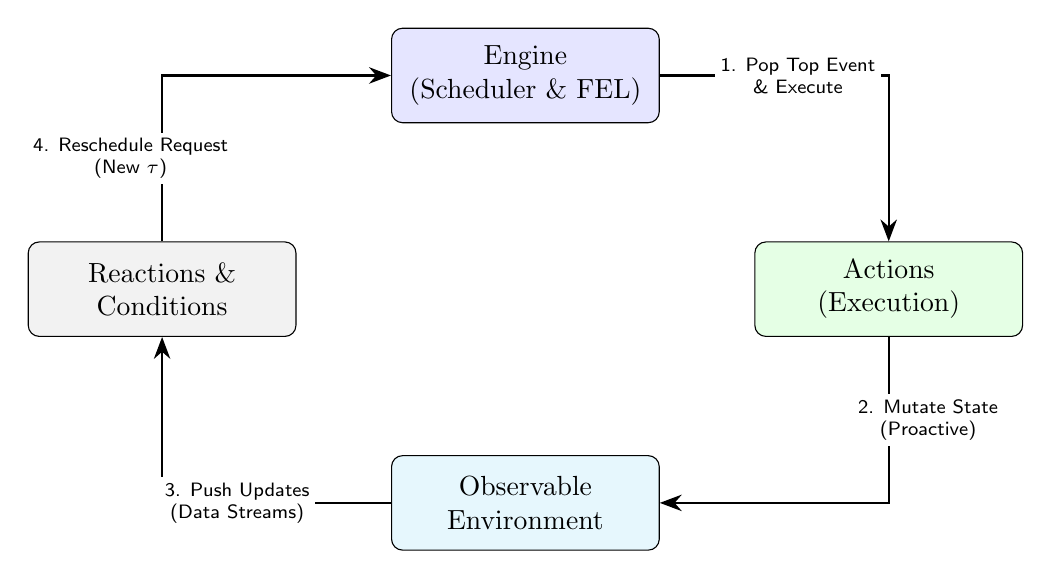
\begin{tikzpicture}[
    box/.style={draw, rectangle, rounded corners, minimum width=3.4cm, minimum height=1.2cm, align=center, fill=gray!10},
    arrow/.style={-{Stealth[scale=1.2]}, thick},
    lbl/.style={font=\sffamily\scriptsize, align=center, fill=white, inner sep=2pt}
]

% Nodes in the exact same diamond layout
\node[box, fill=blue!10] (engine) {Engine \\ (Scheduler \& FEL)};
\node[box, below right=1.5cm and 1.2cm of engine, fill=green!10] (actions) {Actions \\ (Execution)};
\node[box, below left=1.5cm and 1.2cm of engine] (react) {Reactions \& \\ Conditions};
\node[box, below right=1.5cm and 1.2cm of react, fill=cyan!10] (env) {Observable \\ Environment};

% Clean, decoupled circular flow
\draw[arrow] (engine.east) -| node[lbl, near start, xshift=0.3cm] {1. Pop Top Event \\ \& Execute} (actions.north);
\draw[arrow] (actions.south) |- node[lbl, near start, xshift=0.5cm] {2. Mutate State \\ (Proactive)} (env.east);
\draw[arrow] (env.west) -| node[lbl, near start, xshift=-0.5cm] {3. Push Updates \\ (Data Streams)} (react.south);
\draw[arrow] (react.north) |- node[lbl, near start, xshift=-0.4cm] {4. Reschedule Request \\ (New $\tau$)} (engine.west);

\end{tikzpicture}
\end{document}
